\documentclass[runningheads]{llncs}
\usepackage[namelimits]{amsmath} 
\usepackage{amssymb}             
\usepackage{amsfonts}           
\usepackage{mathrsfs}            
\usepackage{graphicx}
\usepackage{amsmath,amssymb} % define this before the line numbering.
\usepackage{ruler}
\usepackage{color}
\usepackage[ruled]{algorithm2e}
\usepackage{multirow}
\usepackage{wrapfig}

\newcommand{\BY}{{Y}}
\newcommand{\BA}{{\mathbf{A}}}
\newcommand{\BX}{{\mathbf{X}}}
\newcommand{\BXs}{{\mathbf{Xs}}}
\newcommand{\BLs}{{\mathbf{Ls}}}
\newcommand{\BD}{{\mathbf{D}}}
\newcommand{\BP}{{\mathbf{P}}}
\newcommand{\BL}{{\mathbf{L}}}
\newcommand{\Bone}{{\mathbf{1}}}
\newcommand{\BU}{{\mathbf{X}}}
\newcommand{\BS}{{\mathcal{S}}}
\newcommand{\BB}{{\mathbf{B}}}
\newcommand{\Bb}{{\mathbf{b}}}
\newcommand{\BR}{{\mathbf{R}}}
\newcommand{\BW}{{\mathbf{W}}}
\newcommand{\BE}{{\mathbf{E}}}
\newcommand{\Be}{{\mathbf{e}}}
\newcommand{\BZ}{{\mathbf{Z}}}
\newcommand{\BM}{{\mathbf{M}}}
\newcommand{\BQ}{{\mathbf{Q}}}
\newcommand{\BT}{{\mathbf{T}}}
\newcommand{\BI}{{\mathbf{I}}}
\newcommand{\T}{{\!\top}}
\newcommand{\Bx}{{\mathbf{x}}}
\newcommand{\By}{{\mathbf{y}}}

\newcommand{\etal}{{et al}}
\newcommand{\etc}{\textit{{etc}}}
\newcommand{\eg}{{e.g.}}
\newcommand{\ie}{{i.e.}}
\newcommand{\w}{{\mathrm{w}}}

\renewcommand{\Lambda}{\varLambda}
\newcommand{\st}{{\,\,\mathrm{s.t.\,\,}}}
\newcommand{\diag}{{\mathrm{diag}}}
\newcommand{\const}{{\mathrm{const.}}}
\newcommand{\trace}{{\mathrm{Tr}}}
\newcommand{\sgn}{{\mathrm{sgn}}}

\usepackage[width=122mm,left=12mm,paperwidth=146mm,height=193mm,top=12mm,paperheight=217mm]{geometry}
\begin{document}
% \renewcommand\thelinenumber{\color[rgb]{0.2,0.5,0.8}\normalfont\sffamily\scriptsize\arabic{linenumber}\color[rgb]{0,0,0}}
% \renewcommand\makeLineNumber {\hss\thelinenumber\ \hspace{6mm} \rlap{\hskip\textwidth\ \hspace{6.5mm}\thelinenumber}}
% \linenumbers
\pagestyle{headings}
\mainmatter
\def\ECCV18SubNumber{1917}  % Insert your submission number here

\title{Supplementary Document:Generative Domain-Migration Hashing for Sketch-to-Image Retrieval} % Replace with your title

\titlerunning{ECCV-18 submission ID \ECCV18SubNumber}

\authorrunning{ECCV-18 submission ID \ECCV18SubNumber}

\author{Anonymous ECCV submission}
\institute{Paper ID \ECCV18SubNumber}


\maketitle
Although the main paper stands on its own, it is still
worthwhile showing more model details and experimental
results. In this supplementary document, we provide:

\begin{itemize}
  \item
  Attention Model Details 

  \item 
  %\vspace{-0.589em}
  	Experiments on the Sketchy dataset

    % We for the first time propose a generative model GDH for the hashing-based SBIR problem. Comparing to existing methods, the generative model can essentially improve the generalization capability by migrating sketches into their indistinguishable counterparts in the natural image domain.
    %We put forward a novel joint end-to-end deep learning method GDH for both category-level
    %and fine-grained SBIR. GDH is able to solve the SBIR problem by 
    %migrating the sketch domain to image domain.
    %To our best knowledge, this work is the first hashing work which transfer
    %sketch domain to image domain with GANs for SBIR problems. And it is the first to incorporates
    %category-level retrieval 
    %and fine-grained retrieval into a unified framework.
   \item
    More illustrative results.
  % \item Guided by an adversarial loss and a cycle consistency loss, the optimized binary hashing codes can preserve the semantic consistency across domains. Meanwhile, training GDH does not require any pairwise correspondence across domains, and thus allows generalized and practical applications.
    %A novel multi-task deep architecture, which collaboratively addresses
%domain-migration and binary coding, is proposed based on discrete alternating iteration.
%Different from previous works contains multi-branch networks, our domain-migration networks are specifically designed. We use the generative network and the hash network for retrieval tasks, which is much simpler and faster.
%Particularly, sketches are fed into the network first to generate the corresponding fake images with little information loss, and the 
%hash function embeds the images and fake images into binary representations. As such, the GDH can better 
%narrow the domain gap between image domain and sketch domain compared to previous SBIR deep nets. And improve the 
%etrieval speed. 
  \item 
  Failure cases and analysis
  % GDH can improve the category-level SBIR performance over the best-performing hashing-based SBIR method DSH \cite{LiuSSLS17} by up to $20.5\%$ on the TU-Berlin Extension dataset, and up to $26.4\%$ on the Sketchy dataset respectively. Meanwhile, GDH can achieve comparable performance with real-valued fine-grained SBIR methods, while significantly reduces the retrieval time and memory cost with binary codes. 
  
 \end{itemize}
 \section{Attention Model Details}
 Since soft attention is now a well-known and conventional
mechanism in deep learning and our attention model
is, to some extent, coherent to the one proposed in \cite{SongYSXH17}
we did not derive the detailed formulation of our attention
model in the main paper.

Considering a convolutional feature map $f$ obtained from the last ResBlock. 
In the first step, the feature maps are mapped into the attention score $s$ by a convolutional
layer with $1 \times 1$ kernel size. Which is defined as:
\begin{equation}\label{eq:equiv1}
\begin{split}
s = relu(w^{T}f + b)
\end{split}
\end{equation}
Next, the attention score $s$ goes through a softmax layer and the output is denoted as p:
\begin{equation}\label{eq:equiv2}
\begin{split}
p = softmax(s)
\end{split}
\end{equation}
A larger value in $p$ corresponds to the foregrounds and
the backgrounds may have a smaller response. Thus, in the
third step, we add a threshold layer to divide the data into
the attended regions and the unattended regions. The $mask$ is
defined as:
\begin{equation}\label{eq:equiv3}
\begin{split}
mask(i,j)=
\begin{cases}
0& p(i,j) \leq \alpha \\
1& p(i,j) \ge \alpha 
\end{cases}
\end{split}
\end{equation}
Where $\alpha$ is the predefined threshold. We set $\alpha = 10^{-5}$ in our experiments. The output of the threshold layer is a binary
mask, with the elements inside be either 0 or 1. The regions
with the value 1 are regarded as the foregrounds or the regions
that are attended to, while other regions are regarded as
background regions.	


 \section{Experiments on the Sketchy database}
 \subsection{Datasets and settings}
  In this section, we present further experimental results on the recently released Sketchy database\cite{sketchy}. %In the original
% experiments presented in the main paper, two datasets: TU-Berlin and Sketchy are chosen for category-level experiments. And two datasets: QMUL-Shoe and QMUL-Chair are chosen for 
 The Sketchy database contains 125 categories with 75,471 sketches of 12,500 object images. In each category, there are 100 object instances. Each instance has one photo and at least 5 corresponding sketches. Following the dataset
partitions in \cite{sketchy,SongYSXH17}, we used 90\% object instances for training and the rest for testing. Specifically, 11,250 of 12,500 photos and
68,175 of 74,425 sketches are used for training. In the provided test data partition, the gallery set contains 1250 photos (10
photos per category) and the test sketch set contains 6250 query sketches (50 sketches per category).

We compare GDH with 3 existing strongest fine-grained SBIR baselines, including : \textbf{AN Siamese:} The base network is AlexNet \cite{KrizhevskySH12}, and it trained with Siamese and classification loss.
\textbf{GN Siamese:}  The base network is GoogLeNet \cite{SzegedyLJSRAEVR15} in a heterogeneous architecture. And the network is also trained with Siamese and classification loss.
\textbf{GN Triplet:}  Same GoogLeNet as the base network is used. The network is trained with Triplet ranking loss and classification loss. Moreover, we compare our model performance with human. \textbf{Human:} This is obtained by asking human participants to browse through the 1,250 gallery photos to find the best match for a given query sketch.\cite{sketchy}

\subsection{Model implementation}
The whole model is same as the model presented in the main paper. And the training strategy follows the algorithm presented in the main paper.
We use the Adam solver \cite{KingmaB14} with a batch size of 32. 
Our balance parameters are set to $\alpha=10^{-5}, \beta=10^{-5}$ and $\lambda=1$.
%\gamma=10^{-5}, \eta=10^{-5}, 
All networks are trained with an initial learning rate $lr=0.0002$. After 25 epochs, we decrease the learning rate of the hashing network $lr\rightarrow 0.1lr$ and terminate the optimization after 30 epochs for both datasets. Our method is implemented by Pytorch with
dual 1080Ti GPUs and an i7-4790K CPU.


\begin{table*}
\tiny
%\scriptsize
\begin{center}
\newcommand{\tabincell}[2]{\begin{tabular}{@{}#1@{}}#2\end{tabular}}
\caption{Accuracy comparison with different fine-grained SBIR baselines on Sketchy}
\resizebox{0.6\textwidth}{!}{
\begin{tabular}{c|c|c}
  \hline
  \multicolumn{2}{c|}{\multirow{1}{*}{\textbf{methods}}} &\multicolumn{1}{|c}{\textbf{Sketchy.acc@1}} \\
\cline{1-2}
  \hline
  \hline
  \multirow{4}{*}{\tabincell{c}{Real-valued\\ vectors}}
  &AN Siamese \cite{sketchy,SongYSXH17}  &0.2136 \\
  &GN Siamese \cite{sketchy,SongYSXH17}   &0.2736  \\
  &GN Triplet \cite{sketchy,SongYSXH17}   &0.3710 \\
  &DSSA \cite{SongYSXH17}   &0.4303 \\
  \hline
  \hline
 \multirow{1}{*}{\tabincell{c}{Binary Codes}}
 %&GDH @ 32-bit &0.286 \\
 &GDH @ 64-bit &\textbf{0.4835} \\
 %&GDH @ 128-bit &0.357 \\
  \hline
  \hline
 \multirow{1}{*}{\tabincell{c}{non-numeric}}
 &Human\cite{sketchy,SongYSXH17}  &0.5427\\
 \hline

  \end{tabular}
  }
\label{table:t1}
\scriptsize

Note that baseline results are copied from the supplementary of \cite{SongYSXH17}.
\vspace{-4ex}
\end{center}
\end{table*}

\subsection{Results and Discussions}
In Table. \ref{table:t1}, we report the top-1 accuracies of GDH over other three methods and human performance on Sketchy dataset for fine-grained SBIR.
Compared to the state-of-the-art real-valued GN Triplet, the 64-bit GDH achieves 11.25\% improvements. Despite binary hashing codes are used,
improved performance over the real-valued state-of-the-art
methods can be observed in Table. \ref{table:t1}. This is because: \textbf{1) Domain-migration strategy}. The generative model can
essentially improve the generalization capability by migrating sketches into
their indistinguishable counterparts in the natural image domain.
 \textbf{2) Specifically designed loss}. The combination of semantic loss and triplet ranking loss, which
preserves category-level information and fine-grained information respectively, exerts positive 
influence on the performance. Different from previous works which use classification loss to preserve the 
category-level information, our semantic loss is more related to binary 
On the other side, the binary codes in
GDH allow much reduced memory costs and retrieval time than the real-valued
approaches.

 \section{Illustrative Results}
 \subsection{Domain-migration networks results on different stage}
 We show more illustrative domain-migration networks results on QMUL-chairs of different training stages in Fig. \ref{fig:gan_results}. 
 It is obviously observed that using sketches
to generate fake images are more difficult than from images to fake sketches. This is because natural images contain much more information than their sketch counterparts,
migrating sketches to natural images is essentially an upsampling process.
 However, the sketch-to-image and image-to-sketch results indicate 
 that our domain-migration networks are capable to transfer domains from both directions.  

 \subsection{Fine-grained SBIR resluts}
We show more illustrative fine-grained SBIR results in
Fig. \ref{fig:fg_results}.  In each example (row), the query
sketch and the top-10 ranked images are shown. Most example queries attain high accuracy among
the first five retrieved candidates.

 \section{failure cases and analysis}
 We do experience failure cases during our experiments. Recalling the fine-grained results
on some unseen query examples, some retrieval results are beyond the top-10 as shown in Fig. \ref{fig:failure_cases}.
We speculate this is because: \textbf{quantization error}. The geometrical morphology and
detailed instance-level characteristic within a category can be much more difficult 
to capture with binary hashing codes than the inter-category discrepancies. We further use the feature without quantization 
to test, results shows that most failure cases change into the top-10.





\begin{figure*}
\vspace{-5ex}
    \centering
    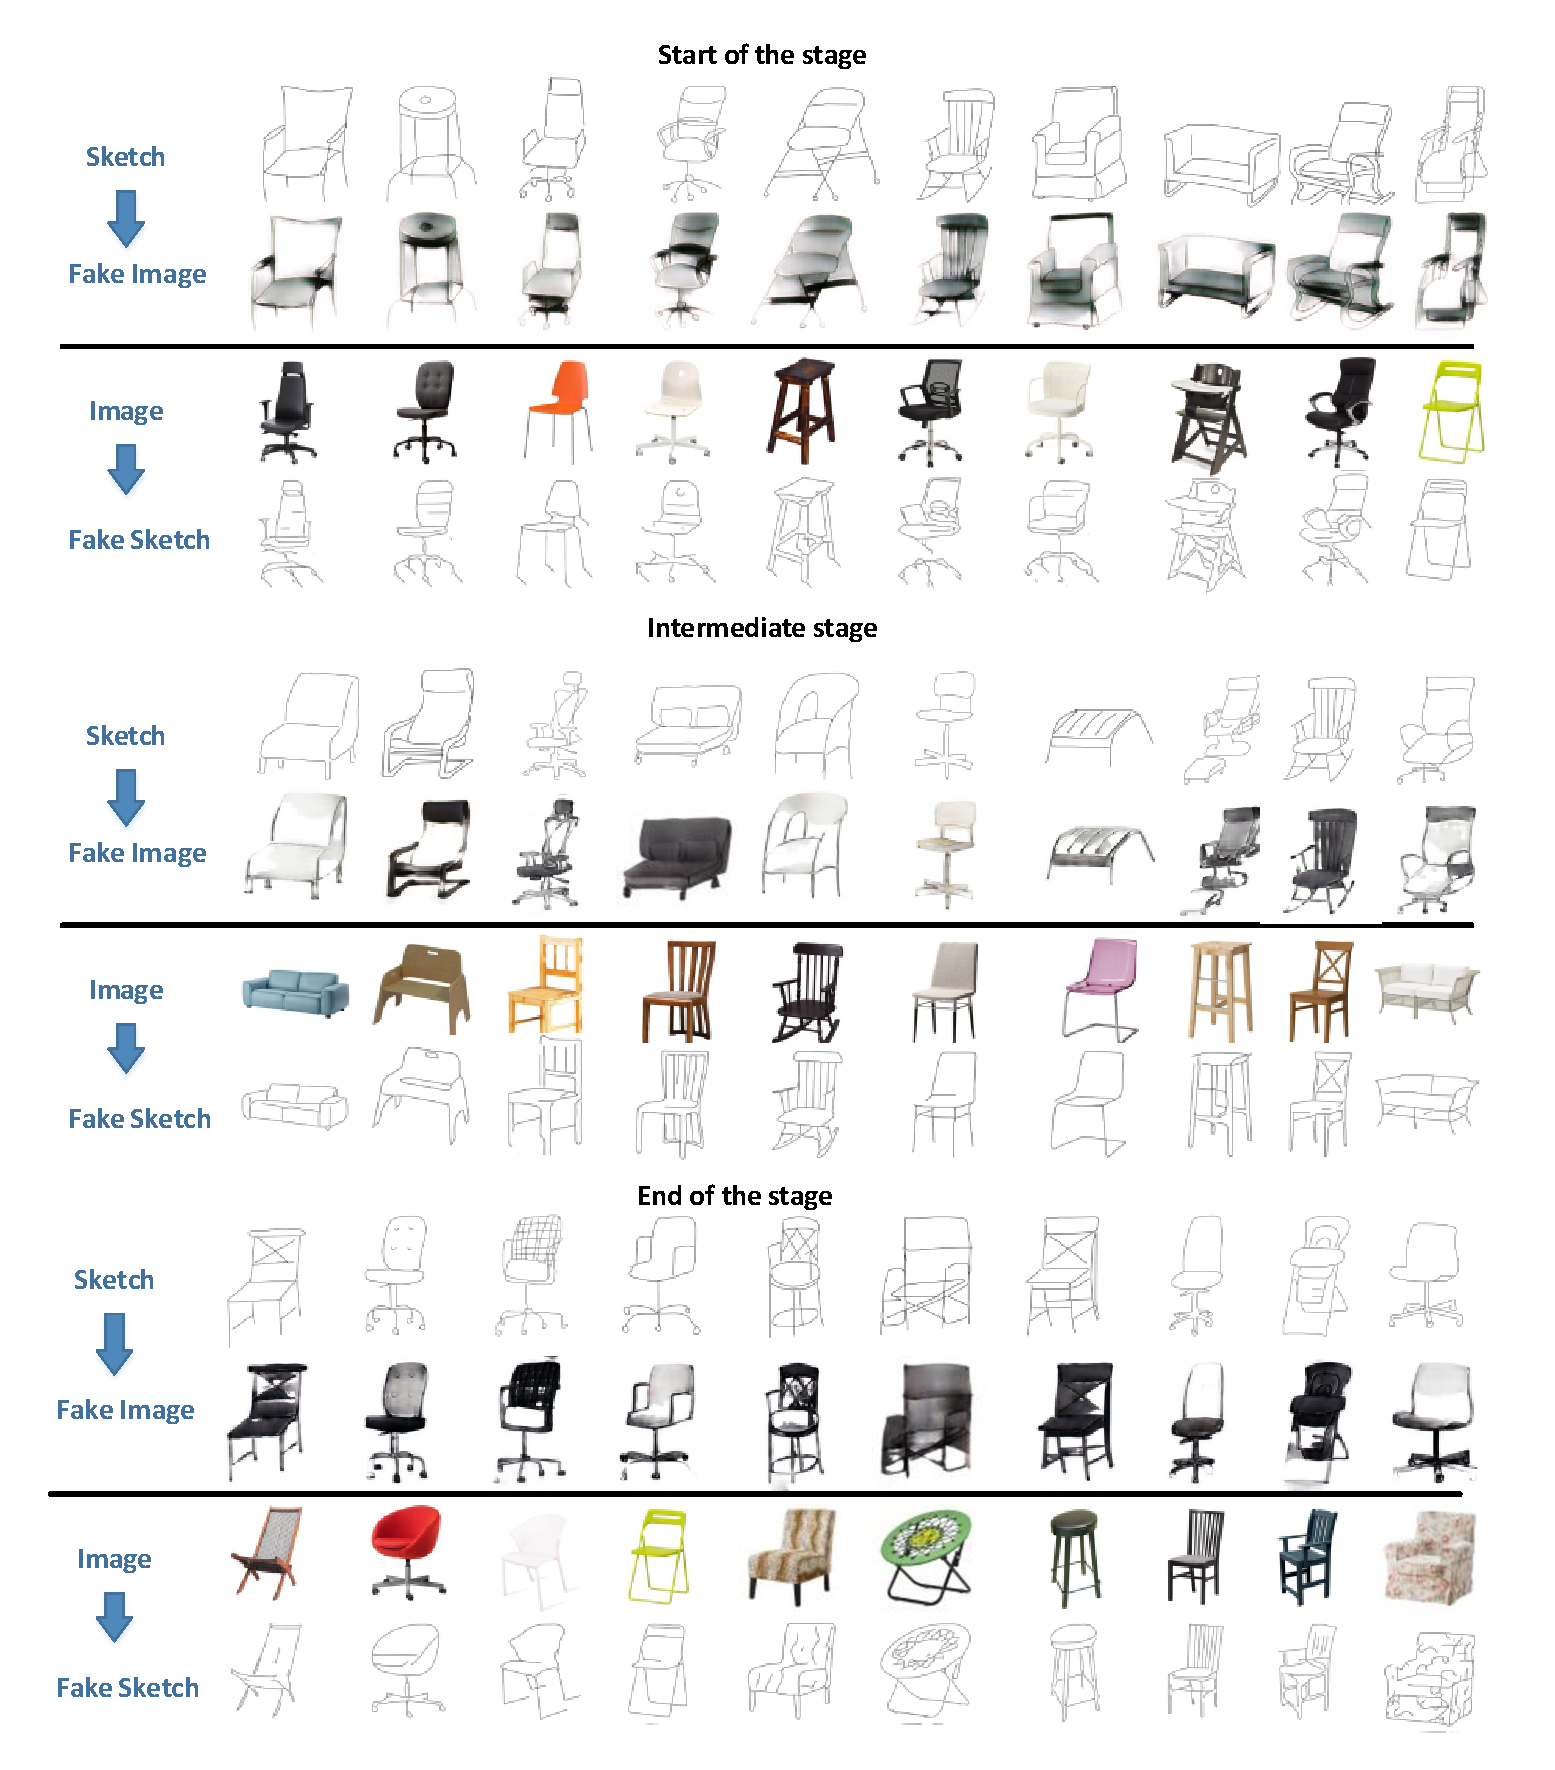
\includegraphics[width = 0.99\textwidth]{figs/gan_results_stage.pdf}
    \vspace{-3ex}
    \caption{Visualization of our domain-migration networks on different stages. In each stage, the first two rows are sketch-
to-image results and the last two rows are image-to-sketch results, which indicates that
our domain-migration networks are capable to transfer domains from both directions.}
    \label{fig:gan_results}
    \vspace{-5ex}
\end{figure*}



\begin{figure*}
\vspace{-5ex}
    \centering
    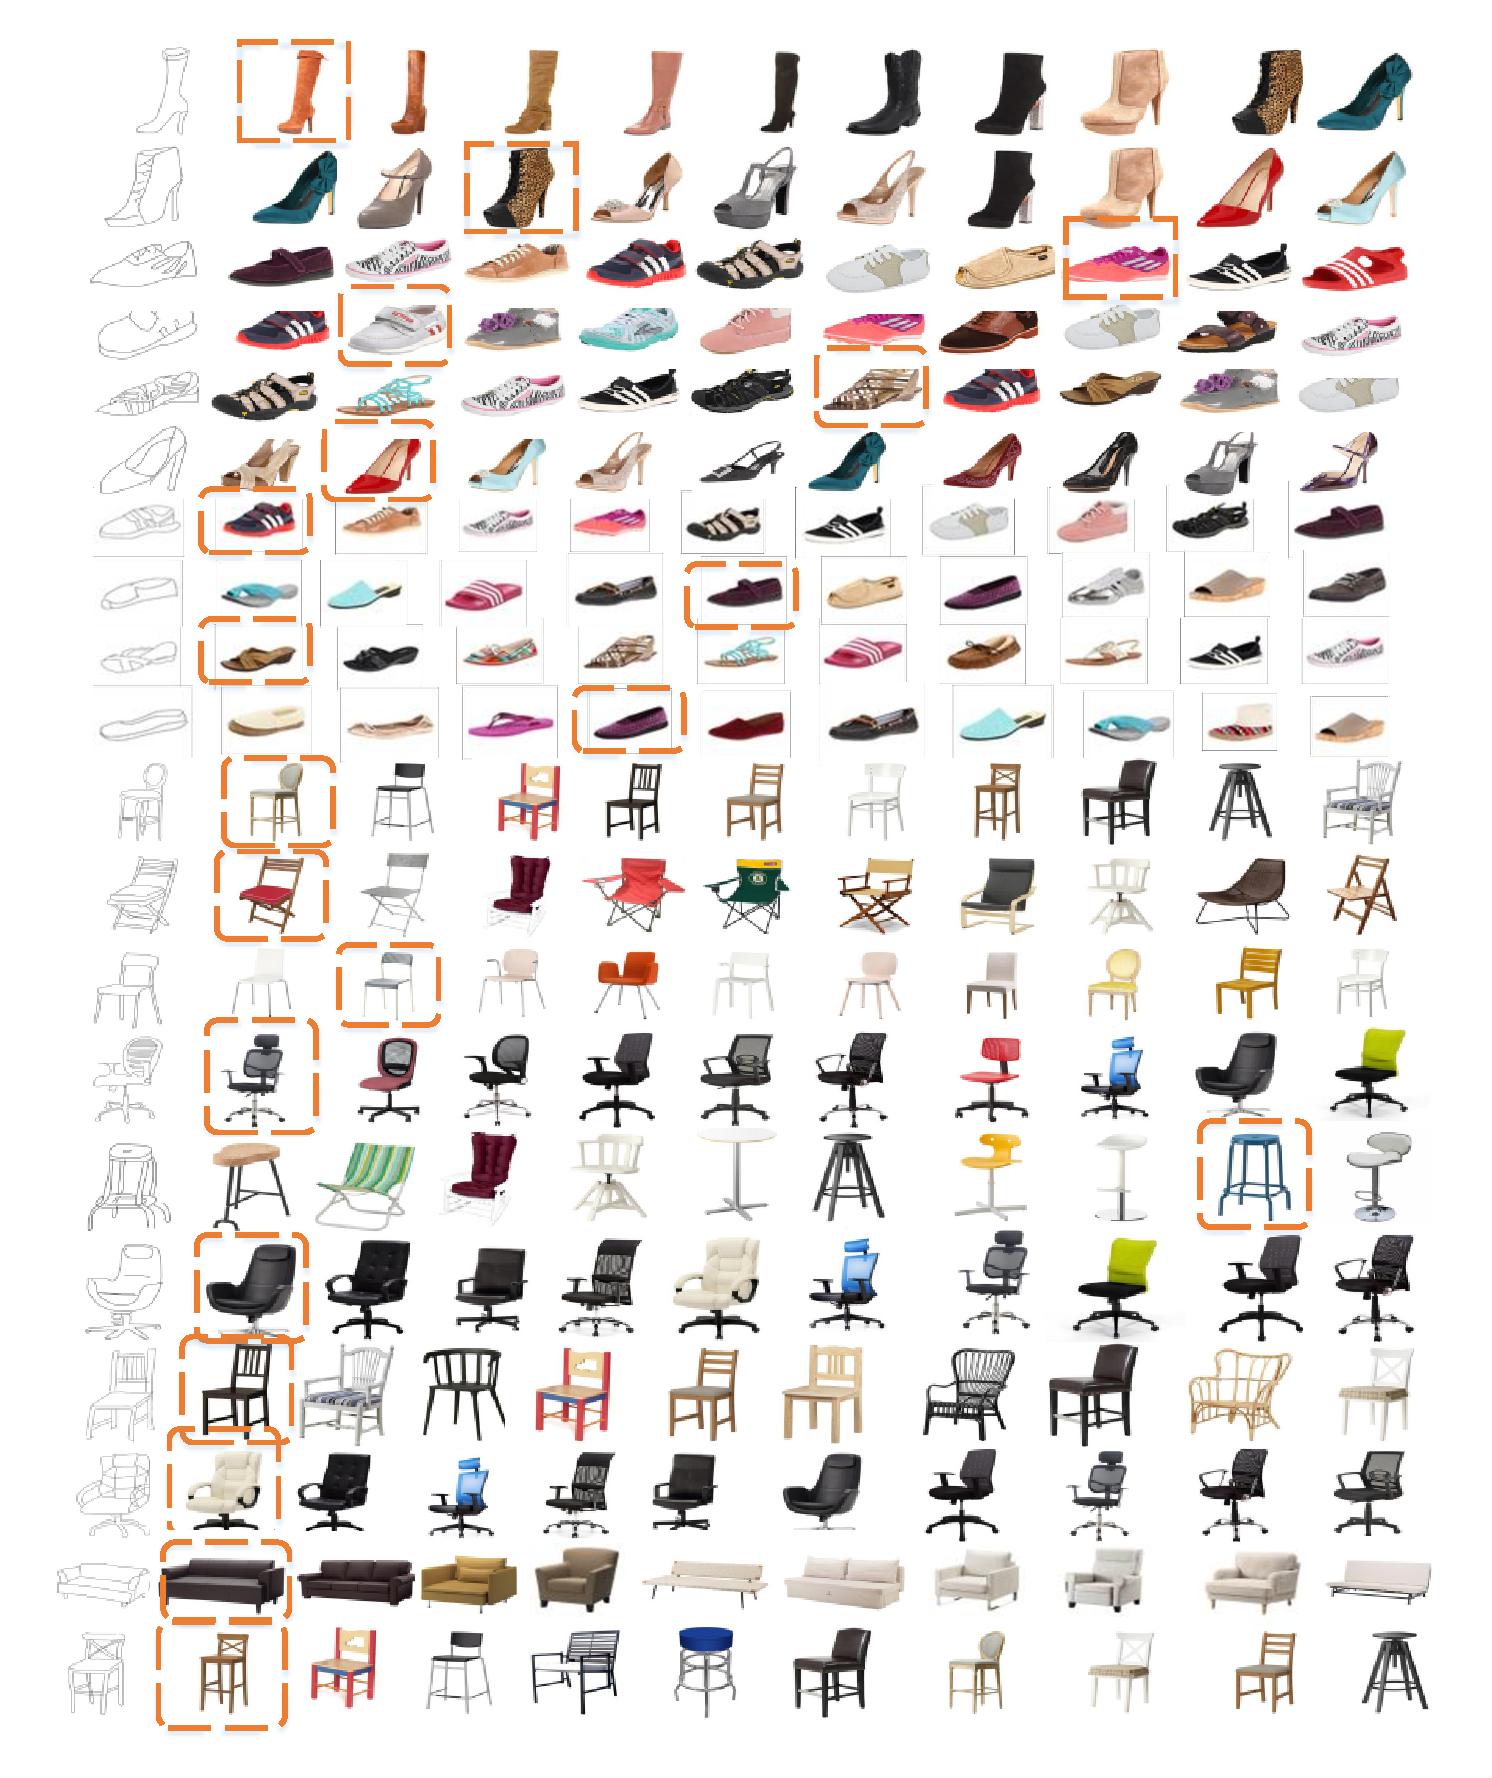
\includegraphics[width = 0.99\textwidth]{figs/fg_results.pdf}
    \vspace{-3ex}
    \caption{Example query sketches with their top-10 retrieval accuracies on the Sketchy
dataset by using 128-bit GDH codes. Orange boxes indicate the groundtruth results.}
    \label{fig:fg_results}
    \vspace{-5ex}
\end{figure*}


\begin{figure*}
\vspace{-5ex}
    \centering
    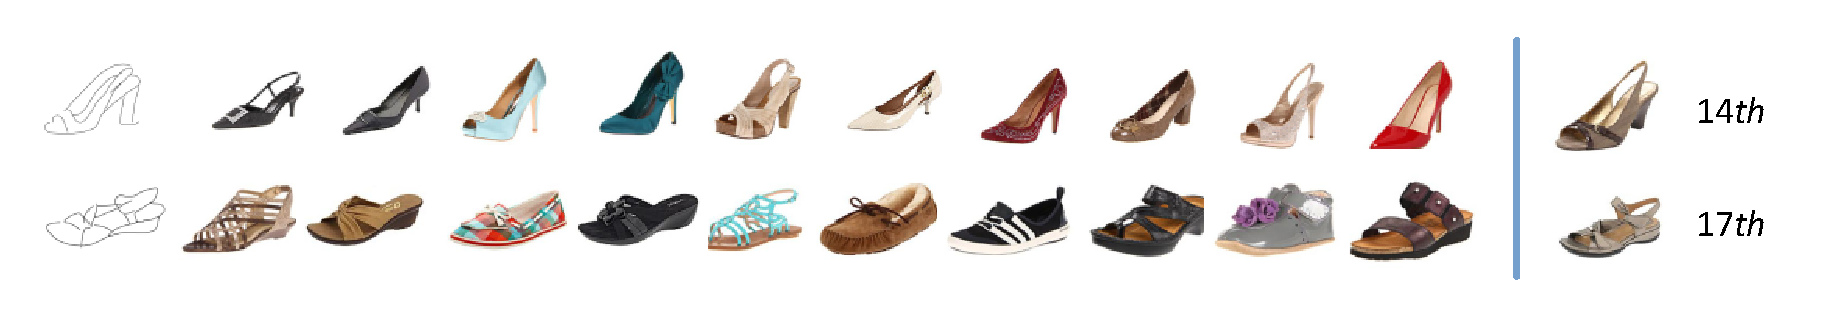
\includegraphics[width = 0.99\textwidth]{figs/failure_cases.pdf}
    \vspace{-3ex}
    \caption{Failure example query sketches with their top-10 retrieval accuracies on the Sketchy
dataset by using 128-bit GDH codes. Top right is the corresponding result and its rank.}
    \label{fig:failure_cases}
    \vspace{-5ex}
\end{figure*}


\bibliographystyle{splncs}
\bibliography{Ref}
\end{document}
